\documentclass[10pt,a4paper]{report}
\pagestyle{headings}
\usepackage{epsfig}

\begin{document}

\title{{\bf A simple coupled terrestrial carbon-physics land scheme for use in a
closed carbon cycle climate model of intermediate complexity}}
\author{Mark Williamson \\ School of Ocean and Earth Science \\
Southampton Oceanography Centre \\ Southampton, UK
\thanks{m.williamson@uea.ac.uk} \and Tim Lenton
\\ School of Environmental Sciences \\ University of East Anglia \\ Norwich, UK
\thanks{t.lenton@uea.ac.uk} \and Ben Adams \\ Department of Animal and Plant Sciences \\
University of Sheffield \\ Sheffield, UK
\thanks{b.j.adams@sheffield.ac.uk} \and John Shepherd \\ School of Ocean and Earth Science \\
Southampton Oceanography Centre \\ Southampton, UK
\thanks{jgs@soc.soton.ac.uk}
\and Andrew Yool \\ School of Ocean and Earth Science \\
Southampton Oceanography Centre \\ Southampton, UK
\thanks{axy@soc.soton.ac.uk}
\and Bob Marsh \\ James Rennell Division \\ Southampton
Oceanography Centre
\\ Southampton, UK
\thanks{rma@soc.soton.ac.uk}}
\maketitle

\begin{abstract}

We have developed a simple land scheme, ENTS (Efficient Numerical
Terrestrial Scheme) for a fully coupled closed carbon cycle climate
model of intermediate complexity, GENIE (1-CBM). The land model
energy and moisture fluxes are coupled to the terrestrial
biogeochemistry and the atmosphere through a number of feedbacks.
This report is to act as a user guide and as comprehensive
documentation for ENTS (M).

In the ENTS model, the land carbon cycle of Lenton (2000)
\cite{Lenton} is enhanced by making it spatially explicit and
incorporating a number of modifications, some of which include a
land hydrological cycle and the effect of water stress on vegetation
carbon following Adams (2003) \cite{Adams}.
\end{abstract}

\tableofcontents

\chapter{ENTS model components}

This section will briefly show the equations that represent the
various processes built into ENTS.

\section{Land radiation}

The land energy balance equations are inspired by the simple energy
balance model that exists in the EMBM of Edwards and Marsh
\cite{Marsh and Edwards} and Weaver {\em et al.} (2001) \cite{Uvic}.

We model a single soil layer for land points. The solar insolation
forcing for the GENIE model is a diurnal average with a seasonal
oscillation. With this forcing and a single soil layer we make the
approximation that the land temperature reaches equilibrium on the
timescale of each call to the land (one ocean timestep, 3.65 days).
A formal justification for this approximation is given in
cite{Williamson}. We therefore solve for $T_{l}$ in the following
equation:
\begin{equation}\label{land temp}
(1-\alpha_{atm})(1-C_{A})(1-\alpha_{s})Q_{SW} =  Q_{LH} + Q_{LW} +
Q_{SH}
\end{equation}
$\alpha_{s}$ is the land albedo, $\alpha_{atm}$ is the atmospheric
albedo (see section \ref{albedo section}) and $C_A = 0.3$ is a
partitioning parameter determining the quantity of radiation
absorbed by dust and moisture in the atmosphere. $Q_{SW}$ is the
incoming short wave solar radiation at the top of the atmosphere.
The heat flux terms on the right hand side of equation (\ref{land
temp}) are given by the following equations and have dimensions of
power per unit area.

The heat flux terms on the right hand side of equation (\ref{land
temp}) are given by the following.

Latent heat
\begin{equation}
Q_{LH}=\rho_{0} L_{\nu} E_{Q}
\end{equation}
Where $\rho_{0}$ is the density of water, $1000$ kg/m$^3$ and
$L_{\nu}=2.50 \times 10^6$ J/kg is the latent heat of vaporization.
$E_{Q}$ is the total evaporation, a combination of evaporation from
bare soil, $E_l$ and evapotranspiration from vegetated areas, $E_t$.
All have units of m/s.

Net longwave radiation flux between the atmosphere and the land
\begin{equation}
Q_{LW}=\varepsilon_{l}\sigma T_{l}^4 - \varepsilon_{a}\sigma
T_{a}^4
\end{equation}
Where $\varepsilon_{l}=0.94$ and $\varepsilon_{a}=0.85$ are the
emissivity of land and atmosphere respectively. $\sigma=5.67\times
10^{-8}$ W/m$^2$/K$^4$ is the Stefan-Boltzmann constant and $T_a$
is the atmospheric temperature.

Sensible heat
\begin{equation}
Q_{SH}=\rho_a C_{H} c_{pa} U (T_l - T_a)
\end{equation}
Where $\rho_a=1.25$ kg/m$^3$ is a constant surface air density,
$c_{pa}=1004$ J/kg/K is the specific heat capacity of air and $U$
is the wind speed in m/s. $C_{H}$ is a transfer coefficient for
heat and is given by
\begin{equation}
C_{H}=\left[\frac{1}{\kappa}\ln(\frac{z_r}{z_0})\right]^{-2}
\end{equation}
Where $\kappa=$0.41 is the Von Karman constant, $z_r$ is a reference
height, the same height at which $U$ is taken, $10$ m, and $z_0$ is
the roughness length of the surface.

The roughness length, $z_0$, has a linear dependence on vegetation
carbon, $C_{\upsilon}$.
\begin{equation}
z_0={\min\{0.001,k_{z}C_{\upsilon}\}}
\end{equation}

All heat fluxes are given in W/m$^2$ and are completely analogous
to those given in C-GOLDSTEIN.

\section{Land hydrology}
Here a new land hydrology scheme is suggested (by TML and MSW)
based on Sellers (1992) \cite{Sellers}.

%The land hydrology draws from the work of Adams (2003) with
%improvements to the transpiration function and some other
%modifications.

Each land grid box has a water reservoir that has a saturated value
of $W_{s}^*$ and a present value of $W_s$. Both have dimensions of
metres. Water is added to the land by precipitation, $P_w$
(dimensions m/s) and removed by evaporation $E$ and runoff $R$:
\begin{equation}
\frac{\partial W_s}{dt}=P_w - E - R
\end{equation}

Evaporation, $E$ is a conglomerate of both Weaver {\em et al.}
(2001) \cite{Uvic} and the approach of Sellers (1992) \cite{Sellers}
and others. If the grid box is below saturation point / field
capacity (i.e. $W_s<W_{s}^*$) then evaporation has a multiplier
$\beta$, which represents the fact that the land surface is less
likely to give up water the drier it becomes. This gives $E$ as
\begin{equation}
E = \beta \frac{\rho_{a} C_W U}{\rho_{0}}(q_s(T_l)-q_a)
\end{equation}
$q_s(T_{l})$ is the saturation specific humidity for land and $q_a$
is the atmospheric surface specific humidity (dimensionless units)
and both are given in Weaver {\em et al.} (2001) \cite{Uvic}.
$C_{W}$ is the transfer coefficient for moisture and we make the
reasonable approximation that $C_W=C_H$. The $\beta$ function is
formulated to give a value between $0$ and $1$ depending on the soil
saturation. If $\beta=1$ then $E$ just reverts to evaporation for a
surface with freely available water. If $W_s<W_{s}^*$ then
\begin{equation}
\beta = \left(\frac{W_s}{W_{s}^*}\right)^4
\end{equation}
and $\beta=1$ if $W_s\geq W_{s}^*$.

%The carbon density function is given by
%\begin{equation}
%C_{\rho}=1 - e^{-k_{17}\frac{C_{\upsilon}}{f_{\upsilon}}}
%\end{equation}
%This function is formulated to saturate at high vegetation
%densities and change rapidly around small changes in vegetation
%density. $k_{17}=0.25$ m$^2$/kgC.

%Vegetation is assumed to be at atmospheric temperature $T_a$
%whereas soil is at $T_l$.
%Canopy conductance ($g_c$ = 1/$r_c$ in
%m/s) is related to stomatal conductance ($g_s$) by a scaling
%factor ($f_{par}$):
%\begin{equation}
%g_c = k_Q g_s f_{par}
%\end{equation}
%Where $k_Q=2.88 \times 10^{-5} $ [check that this doesn't need
%changing] converts canopy conductance from units of
%mol$CO_2$/m$^2$/s to units of m/s (it includes the factor of 1.6
%difference in diffusivity of $H_2O$ and $CO_2$). The scaling
%factor $f_{par}$ is based on exponential decay of incident
%photosynthetically active radiation (PAR) through the canopy:
%\begin{equation}
%f_{par} = \frac{1-exp(-kL)}{k}
%\end{equation}
%Where $k$=0.5 is the canopy light extinction coefficient (from
%TRIFFID, where it is identical for all five plant functional
%types) and L is leaf area index (LAI) given by:
%\begin{equation}
%L = \frac{aC_{\upsilon}}{f_{\upsilon}}
%\end{equation}
%We assume LAI varies linearly with the areal carbon density of
%vegetation $C_{\upsilon}$/$f_{\upsilon}$ (in kgC/m$^2$
%vegetation)[not sure about the validity of this], which for
%constant volumetric density over the vegetated area would be
%equivalent to height. LAI typically ranges up to 9 so we set a =
%0.75 [worth experimenting with this parameter - could ignore it
%i.e. a = 1?].
%The transpiration term (in m/s) is given by
%\begin{equation}
%Q = k_Q g_c (q_s(T_a)-q_a)
%Q = \frac{k_{3} \mu P}{\rho_0 }
%\frac{k_{33}(q_s(T_a)-q_a)}{(pCO_2-k_{13})(1+\frac{(q_s(T_a)-q_a)}{k_{34}})}
%\end{equation}

Runoff, $R$ (in m/s) can be thought of as the `overflow' of the
water buckets. If during a timestep, $\delta t$, $W_s>W_{s}^*$
then the runoff will be
\begin{equation}
R=\frac{1}{\delta t}(W_{s}-W{s}^*)
\end{equation}
Where $R$ is always $\geq 0$. This term adds water to an ocean
grid box determined by a runoff matrix already present in
C-GOLDSTEIN.

%Runoff, $R$ has been parameterised as a discrete process, the
%amount of runoff being linearly dependent on the fraction of the
%grid box's fullness.
%\begin{equation}
%R = \frac{k_7}{\rho_0} \frac{W_s}{W_{s}^*}
%\end{equation}
%Where $k_{7}=1.18\times 10^{-5}$ kg/m$^2$/s. This term adds water
%to an ocean grid box determined by a runoff matrix already present
%in C-GOLDSTEIN.

Lastly, each grid box's water reservoir saturation value $W_{s}^*$
can either be constant (e.g. 0.2 m) or have a linear dependence on
soil carbon, $C_s$ i.e.
\begin{equation}
W_{s}^* =k_9 + k_{10} C_{s}
\end{equation}
This represents the difference between the water holding capacity
of a desert (sand) and a forest (soil). $W_{s}^*$ has a maximum
value of 0.45 m.

\section{The carbon cycle}

The land carbon cycle follows a similar structure as Lenton (2000)
\cite{Lenton} and Adams (2003) \cite{Adams} with revised
temperature responses of photosynthesis, plant respiration, and
soil respiration. The water stress function is also revised.

The land can store carbon in one of two ways in the model, either
in the soil or in vegetation. Each grid box has its own vegetation
($C_{\upsilon}$) and soil carbon ($C_s$) reservoirs. All the
reservoirs have units of kgC/m$^2$ and all fluxes have units of
kgC/m$^2$/yr. Vegetation removes carbon from the atmosphere
through photosynthesis, $P$, and adds carbon to the atmosphere
through plant respiration, $R_{\upsilon}$. Vegetation also loses
carbon to the soil reservoir, through leaf litter, $L$. Finally,
$C_s$ loses carbon to the atmosphere by soil respiration, $R_s$.
The state of the vegetation is described by both its carbon
density $C_{\upsilon}$ and the fraction of the grid box it covers,
$f_{\upsilon}$. The vegetation carbon reservoir evolves according
to
\begin{equation}
\frac{\partial C_{\upsilon}}{\partial t} = P - R_{\upsilon} - L
\end{equation}
The soil reservoir according to
\begin{equation}
\frac{\partial C_{s}}{\partial t} = L - R_s
\end{equation}
The carbon flux to the atmosphere from the land is given by
\begin{equation}
\frac{\partial C_{a}}{\partial t} = R_s + R_{\upsilon} - P
\end{equation}
%Each of the carbon flux terms are given by the following equations:

%Photosynthesis is first calculated at the leaf level and then
%scaled to the canopy and to land area. Leaf net photosynthesis
%($A$) (i.e. gross photosynthesis minus photo-respiration) is given
%by:
%\begin{equation}
%A= k_{18} f_1(CO_2) f_2(W_s) f_3(T_a)
%\end{equation}
Net photosynthesis, $P$, (i.e. gross photosynthesis minus
photo-respiration) is given by:
\begin{equation}
P= k_{18} f_1(CO_2) f_2(W_s) f_3(T_a) f_{\upsilon}
\end{equation}

This is a product of three functions representing the carbon dioxide
fertilization effect $f_1(CO_2)$, water stress on vegetation
$f_2(W_s)$, and air temperature dependance of growth $f_3(T_a)$. The
constant $k_{18}$ in kgC/m$^2$ leaf/yr is a baseline leaf
photosynthesis rate. $f_{\upsilon}$ is the vegetated fraction.

If $pCO_2>k_{13}$ then
\begin{displaymath}
f_1(CO_2)=\frac{1}{k_{19}}\frac{pCO_2-k_{13}}{pCO_2-k_{13}+k_{14}}
\end{displaymath}
Otherwise $f_1(CO_2)=0$. $pCO_2$ is the atmospheric concentration of
CO$_2$ in ppmv, $k_{13}=29$ ppmv and $k_{14}=145$ ppmv (from Lenton,
2000). $k_{19}=(280-k_{13})/(280-k_{13}+k_{14})=0.6338$ normalizes
the $CO_{2}$ response.

%$k_{12}=(280-k_{13}+k_{14})/(280-k_{13})=1.5777$ is a normalising constant.
%If $k_{15}\leq W_s \leq k_{16}$ then
%\begin{displaymath}
%f_2(W_s)=\frac{1}{1+e^{-k_{15}(W_s-k_{16})}}
%f_2(W_s)=\frac{W_s -k_{15}}{k_{16}-k_{15}}
%\end{displaymath}
%If $W_s < k_{15}$ then $f_2(W_s)=0$ and if $W_s > k_{16}$ then
%$f_2(W_s)=1$. The constants are $k_{15}=0.03$ m and $k_{16}=0.1$
%m.

If $\frac{1}{2}W_s^* \leq W_s \leq \frac{3}{4} W_s^*$ then
\begin{displaymath}
f_2(W_s)=\frac{4 W_s}{W_s^*}-2
\end{displaymath}
If $W_s < \frac{W_s^*}{2}$ then $f_2(W_s)=0$ and if $W_s > \frac{3
W_s^*}{4} $ then $f_2(W_s)=1$.

The temperature response of photosynthesis is based on that of the
maximum carboxylation rate of Rubisco, with an additional cut-off
term at sub-zero temperatures (following MOSES2/TRIFFID). However,
we combine two temperature response functions in order to capture
the response of both high and low latitude vegetation types:
\begin{displaymath}
f_3(T_a)=\mathrm{f_3}(T_a)+\mathrm{f_{3a}}(T_a)
\end{displaymath}
The two functions making up $f_3(T_a)$ are given by
\begin{displaymath}
\mathrm{f_3}(T_a)=\frac{2.0^{0.1(T_a-T_{ref})}}{(1+e^{0.3(T_a-k_{11})})(1+e^{-0.3(T_a-k_{12})})}
\end{displaymath}
\begin{displaymath}
\mathrm{f_{3a}}(T_a)=\frac{2.0^{0.1(T_a-T_{ref})}}{(1+e^{0.6(T_a-k_{11a})})(1+e^{-0.3(T_a-k_{12})})}
\end{displaymath}
Where $T_{ref}=298.15$K, $k_{11}=309.15$K, $k_{11a}=283.15$K and
$k_{12}=268.15$K.

%$k_{a}=2.0$
%$k_{17}$=1.037 normalizes the response at 298.15K [ignored].
%If $k_{11}<T_a<k_{k12}$ then $f_{T_a}$ is given by
%\begin{displaymath}
%f_{T_a}=(T_a-k_{11})^2(k_{12}-T_a)
%\end{displaymath}
%Otherwise $f_{T_a}=0$. $k_{11}=268$ K and $k_{12}=318$ K.

%To scale from leaf to canopy photosynthesis (following TRIFFID) we
%use the factor $f_{par}$ (defined in the section above), based on
%exponential decay of incident photosynthetically active radiation
%(PAR) through the canopy. To convert from canopy photosynthesis
%(kgC/m$^2$ vegetation) to photosynthesis per unit land area
%(kgC/m$^2$ land) we must also multiply by $f_{\upsilon}$:
%\begin{equation}
%P= A f_{par} f_{\upsilon}
%\end{equation}

The vegetation fraction, $f_{\upsilon}$, is made as a simple
saturating function of vegetation carbon. This formulation is
likely to change. Vegetation fraction is given by
\begin{equation}
f_{\upsilon}=1 - e^{-k_{17}C_{\upsilon}}
\end{equation}
Vegetation respiration depends on the air temperature and the
amount of vegetation present (following Lenton, 2000):
\begin{equation}
R_{\upsilon}=\frac{k_{24}}{k_{25}} f_4(T_a) C_{\upsilon}
\end{equation}
where  $k_{24}$ is a vegetation respiration rate (/yr) and $k_25$ is
a normalising constant.
\begin{displaymath}
f_4(T_a)=e^{\frac{k_{20}}{R T_a}}
\end{displaymath}
where $k_{20}=54830$ J/mol is an activation energy, and $R=8.314$
J/mol/K is the universal gas constant.

%R_{\upsilon}=\frac{k_{24}}{k_{25}}[\frac{e^{k_{20}(T_a-k_{21})}}
%{1+e^{k_{22}(T_a-k_{23})}}] C_{\upsilon}
%Where $k_{20}=0.075$, $k_{21}=293$ K, $k_{22}=0.2$, $k_{23}=309$
%K, $k_{24}=0.092$ /yr and
%$k_{25}=e^{k_{20}(288-k_{21})}/(1+e^{k_{22}(288-k_{23})})$ is a
%normalising factor i.e. $R_{\upsilon}=k_{24} C_{\upsilon}$ at the
%optimum atmospheric temperature, $T_a=288$ K.

The quantity of carbon lost by the vegetation to the soil via leaf
litter is related to the amount of vegetation.
\begin{equation}
L=k_{26}C_{\upsilon}+ \varepsilon(P-R_{\upsilon})
\end{equation}
Where $k_{26}$ is in units of /yr, a turnover rate. $\varepsilon$
represents self shading. It is given by
\begin{equation}
\varepsilon=\frac{1}{1+e^{k_{16}-C_\upsilon}}
\end{equation}
This equation implies that all new production is channeled into leaf
litter when $\epsilon \rightarrow 1$. This occurs when $f_\upsilon
\rightarrow 1$.

Carbon lost to the atmosphere soil respiration is dependent on the
land temperature $T_l$ and the amount of carbon in the soil
reservoir, $C_s$:
\begin{equation}
R_s=\frac{k_{29}}{k_{30}} f_{5,6}(T_l) C_s
\end{equation}
Where $k_{29}$ is the soil respiration rate (/yr), and $k_{30}$ is
a normalising constant. Above freezing, for $T_l\geq 273.15$ K:
\begin{displaymath}
f_5(T_l)=e^{-k_{31}/(T_l-k_{32})}
\end{displaymath}
from Lloyd and Taylor (1994), where $k_{31}=308.36$ K,
$k_{32}=227.13$ K. Below freezing, soil respiration rate is
assumed to have a constant $Q_{10}$ temperature sensitivity, for
$T_l<273.15$ K:
\begin{displaymath}
f_6(T_l)=k_{0} Q_{10}^{0.1(T_l-T_{0})}
\end{displaymath}
where $T_{0}=273.15$ K, $k_{0}=f_5(T_{0})$, and $Q_{10}=e^{10
k_{31}/(T_{0}-k_{32})^2}=4.289$. (This prevents unrealistic
blow-up of the soil reservoir as $T_l$ approaches $k_{32}$ in
$f_5$.)

%Finally, the other variable describing the state of the
%vegetation, the fractional cover of vegetation in each grid box
%evolves according to
%\begin{equation}\label{fv change}
%\frac{\partial f_{\upsilon}}{\partial t} = \Psi^+ - \Psi^-
%\end{equation}
%The two terms in equation (\ref{fv change}) represent plant death,
%the rate of decrease of vegetation area, $\Psi^-$ and the rate of
%increase of plant area, $\Psi^+$. These two terms are given by
%\begin{equation}
%\Psi^+=\alpha f_{\upsilon}(1-f_{\upsilon})
%\end{equation}
%\begin{equation}
%\Psi^-=k_{28}f_{\upsilon}
%\end{equation}
%Where $k_{28}=0.1$ /yr. $\alpha$ is the potential rate of increase
%and is given by $\alpha =k_{27}(P-R_{\upsilon})C_{\rho}$ if
%$P>R_{\upsilon}$ or $\alpha=0$ otherwise, where $k_{27}=4.1059
%\times 10^{-14}$ gridbox/mol.

\section{Elevation}

The ENTS model includes altitude effects. At startup, the model
reads in a height above sea-level for each land point and alters the
sea-level air temperature calculated in C-GOLDSTEIN according to a
lapse rate. The equation for the air temperature over land at height
$z$ (in metres) is given by
\begin{equation}
T_{a}(z)=T_{a}(0)+\Gamma z
\end{equation}
Where $\Gamma=-6.5$ K/km. When this effect is included by setting
the {\tt orogswitch} in {\em goin\_ents} to 1, altitude effects are
also included in the calculation of evaporation, outgoing planetary
longwave radiation flux and sensible heat flux (see Weaver {\em et
al.} (2001) \cite{Uvic} for these equations). Figure \ref{elevation}
shows the height of each grid box.

\begin{figure}
\centerline{\scalebox{0.6}{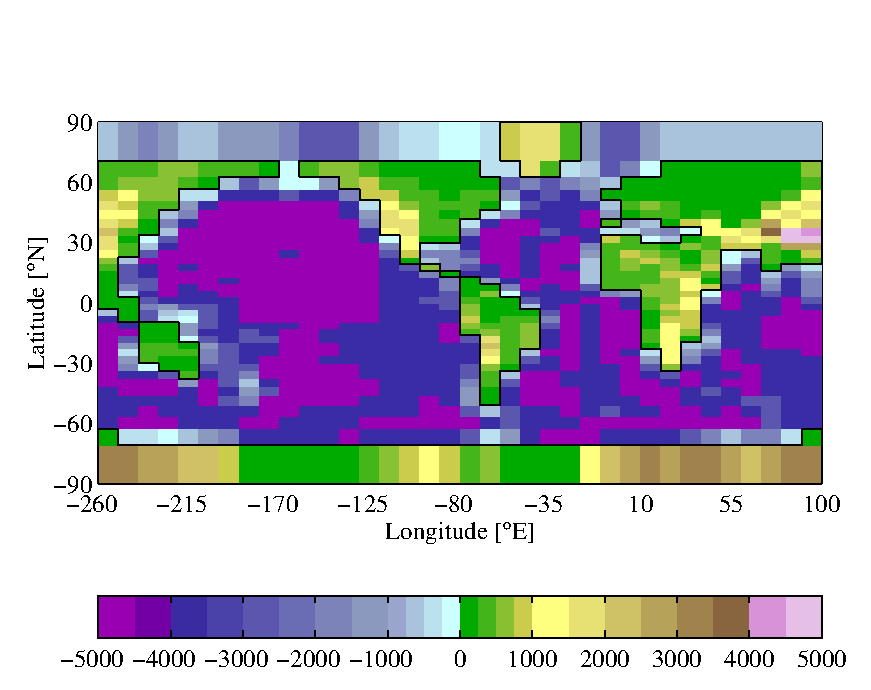
\includegraphics{elevation.eps}}}
\caption{Height in metres of each grid box}\label{elevation}
\end{figure}

\section{Albedo}\label{albedo section}

When ENTS is compiled together with C-GOLDSTEIN plus any other
component, the albedo scheme in C-GOLDSTEIN is replaced in all
models by ENTS's own scheme. In C-GOLDSTEIN albedo is prescribed by
latitude from a sinusoidal planetary albedo function (a planetary
albedo is the resulting albedo from all the other individual albedos
of clouds, zenith angle effects and surface colour). This is
overwritten by ENTS to give a separate surface albedo and a separate
atmospheric albedo.

We calculate the prescribed fields of atmospheric albedo by making
the approximation that there are two reflective layers that make up
the planetary albedo, one at the top of the atmosphere, the
atmospheric albedo and one at the air-land/air-sea interface which
is suitable for our 1 layer atmosphere. Neglecting multiple
reflections and absorptions this gives the planetary albedo,
$\alpha_p$, as
\begin{equation}\label{planet albedo}
\alpha_p = \alpha_{atm} + \alpha_s (1-\alpha_{atm})(1-C_A)
\end{equation}
Where $\alpha_s$ is the surface albedo taken from the prescribed
data sets of Matthews \cite{Matthews} and the ocean albedo
calculation (see later on in this section). $C_A$ is the absorption
in the atmosphere. Planetary albedo is determined from NCEP long
term monthly mean reanalysis fluxes of solar radiation at the top of
the atmosphere.
\begin{equation}
\alpha_p=\frac{Q_{SW}^{\uparrow}}{Q_{SW}^{\downarrow}}
\end{equation}
$Q_{SW}^{\uparrow}$ is the upward solar flux at the top of the
atmosphere and $Q_{SW}^{\downarrow}$ is the downward solar flux at
the top of the atmosphere. The global annual mean planetary albedo
is 0.377 from the NCEP fields.

We calculate atmospheric albedo by rearranging equation (\ref{planet
albedo}).
\begin{equation}
\alpha_{atm}=\frac{\alpha_p - \alpha_s(1-C_A)}{1 - \alpha_s(1-C_A)}
\end{equation}

A parameterizations of cloud albedo was attempted using the
available EMBM variables but was unsuccessful. To represent a
complex process like this our simple atmosphere does not have enough
variables.

The terrestrial surface albedo is dependent on what the surface is
i.e. snow, sea-ice, vegetation, bare soil or sand. The terrestrial
surface albedo is a function of vegetation and soil carbon. For a
snow free gridbox, the terrestrial surface albedo is
\begin{equation}
\alpha_s=f_{\upsilon}\alpha_{\upsilon} +
(1-f_{\upsilon})\alpha_{soil}
\end{equation}
Where $\alpha_{\upsilon}=0.1$, the albedo of vegetation and
$\alpha_{soil}$ is given by
\begin{equation}
\alpha_{soil}=(\alpha_{peat}-\alpha_{sand})\frac{k_{10}C_s}{k_8-k_9}+\alpha_{sand}
\end{equation}
Where $\alpha_{peat}=0.11$ and $\alpha_{sand}=0.3$. This function
has a minimum value of $\alpha_{peat}$. If snow is present the
terrestrial surface is calculated as
\begin{equation}
\alpha_s^{snow}=(\alpha^{snow}-\alpha_{\upsilon}^{snow})e^{-k_7
C_{\upsilon}}+\alpha_{\upsilon}^{snow}
\end{equation}
Where $\alpha_{\upsilon}^{snow}=0.3$ is the snow covered
vegetation albedo and $\alpha^{snow}=0.8$ is the albedo of a snow
covered flat surface.

Calculation of the ocean surface albedo: Ocean albedo is basically
Fresnel reflection. Water is a transparent, non-magnetic medium and
the reflectivity of the ocean is dependent on the refractive index
contrast across the ocean-atmosphere interface and the incidence
angle of the incoming light, the solar zenith angle. The refractive
index of sea-water is pretty much constant ($n\approx 1.339$) for
the visible wavelength band but the solar zenith angle, $Z$, varies
with latitude, $\phi$ and the time of year. C-GOLDSTEIN does not
resolve the diurnal cycle so the daily average ocean albedo needs to
be calculated. It is given by
\begin{equation}
\alpha_{ocean}=\frac{\int^{H}_{0} R(Z) \cos Z dh}{\int^H_0 \cos Z
dh}
\end{equation}
$R(Z)$ is the reflectivity of the ocean based on an empirical
formula (Briegleb {\em et al.}, 1986 \cite{Ramanathan}, but can
also be calculated from electromagnetic theory, the Fresnel
equations) and $H$ is the angular half-length of the day (see
Peixoto and Oort (1991) \cite{P+O}). The cosine of the solar
zenith angle is given by
\begin{equation}
\cos Z = \sin \phi \sin \delta + \cos \phi \cos \delta \cos h
\end{equation}
Where $\phi$ is the latitude, $\delta$ is the declination of the
sun and $h$ is the hour angle from the local meridian where $h=0$.

This gives $H$ as
\begin{equation}
H = \cos^{-1}(- \tan \phi \tan \delta)
\end{equation}

$R(Z)$ is given by the following expression:
\begin{displaymath}
R(Z)=R_{specular}(Z)+R_{diffusive}
\end{displaymath}
\begin{equation}
R_{specular}(Z)=\frac{2.6\times 10^{-2}}{(\cos
Z)^{1.7}+0.065}+0.15(\cos Z -0.1)(\cos Z-0.5)(\cos Z-1.0)
\end{equation}
$R_{specular}$ is the specular reflection and $R_{diffusive}$ is the
diffusive reflection modeled as a constant ($=0.06$).

The ocean albedo is calculated via a numerical integration
algorithm (an adaptive extended trapezium rule) for each latitude
and at each time of the year at the initialization stage of the
run and stored in an array.

Figure \ref{albedo} shows the planetary albedo and figure
\ref{albedo_surf} shows the surface albedo of each grid box.

\begin{figure}
\centerline{\scalebox{0.6}{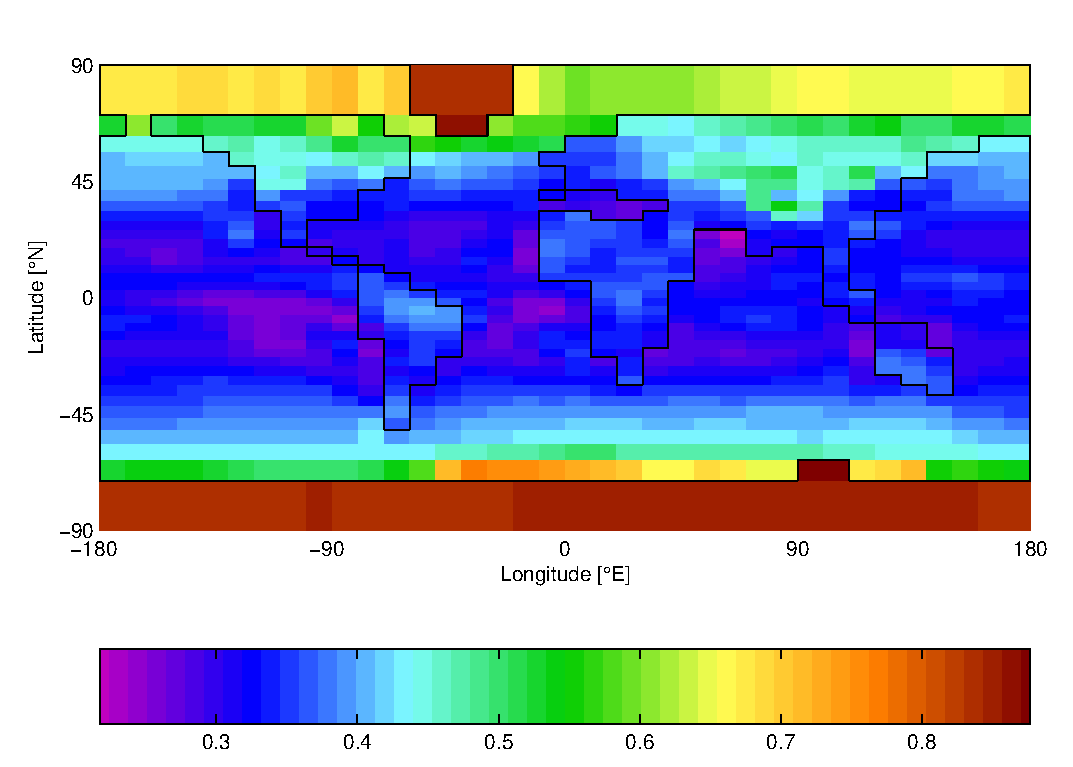
\includegraphics{albedo.eps}}}
\caption{Annual average planetary albedo}\label{albedo}
\end{figure}

\begin{figure}
\centerline{\scalebox{0.6}{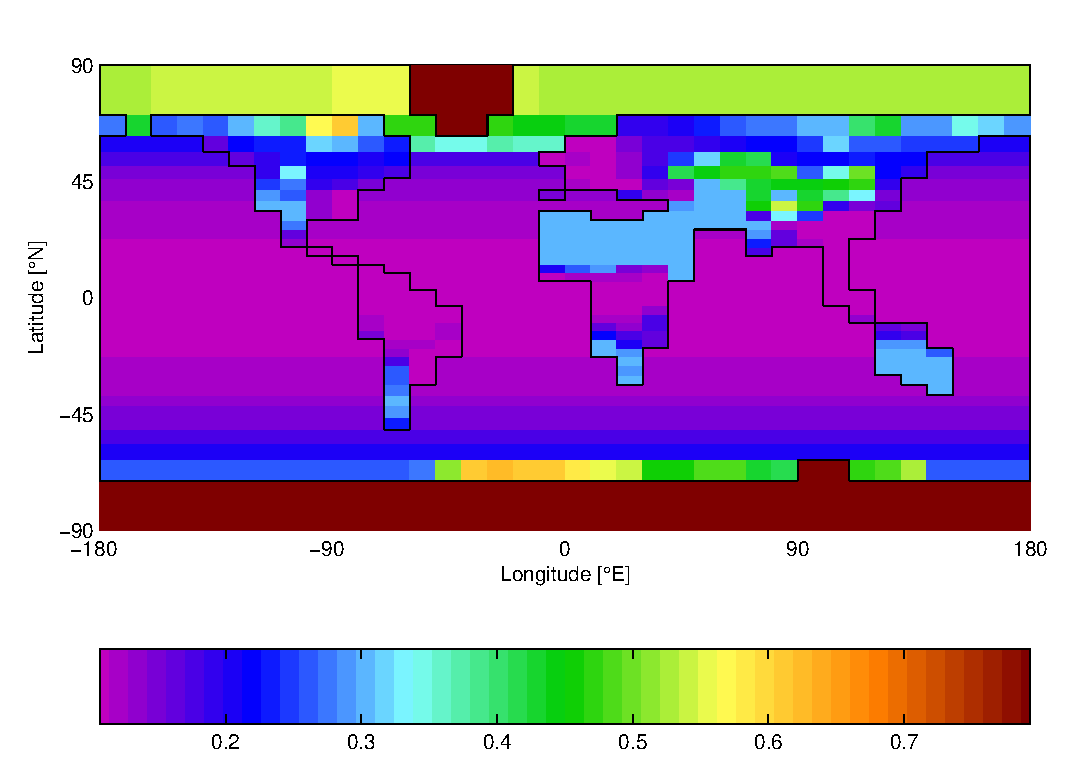
\includegraphics{albedo_surf.eps}}}
\caption{Annual average surface albedo}\label{albedo_surf}
\end{figure}

\section{Snow}

In ENTS there is a simple parameterizations of snow albedo feedback
which can be switched on or off using {\tt snowswitch} in {\em
goin\_ents}. Whether or not the albedo feedback is switched on the
model will calculate fractional snow cover for each land grid box.
Snow will be found lying in a land grid box that fulfills the
following conditions: $T_{a}\leq -5^{o}$C and $T_{l}\leq -5^{o}$C
and precipitation must be greater than zero. The snow will remain on
the grid box until either $T_{a}$ or $T_{l}$ are larger than
$-5^{o}$C. Figure \ref{snow} shows the annual average fractional
snow cover.

\begin{figure}
\centerline{\scalebox{0.6}{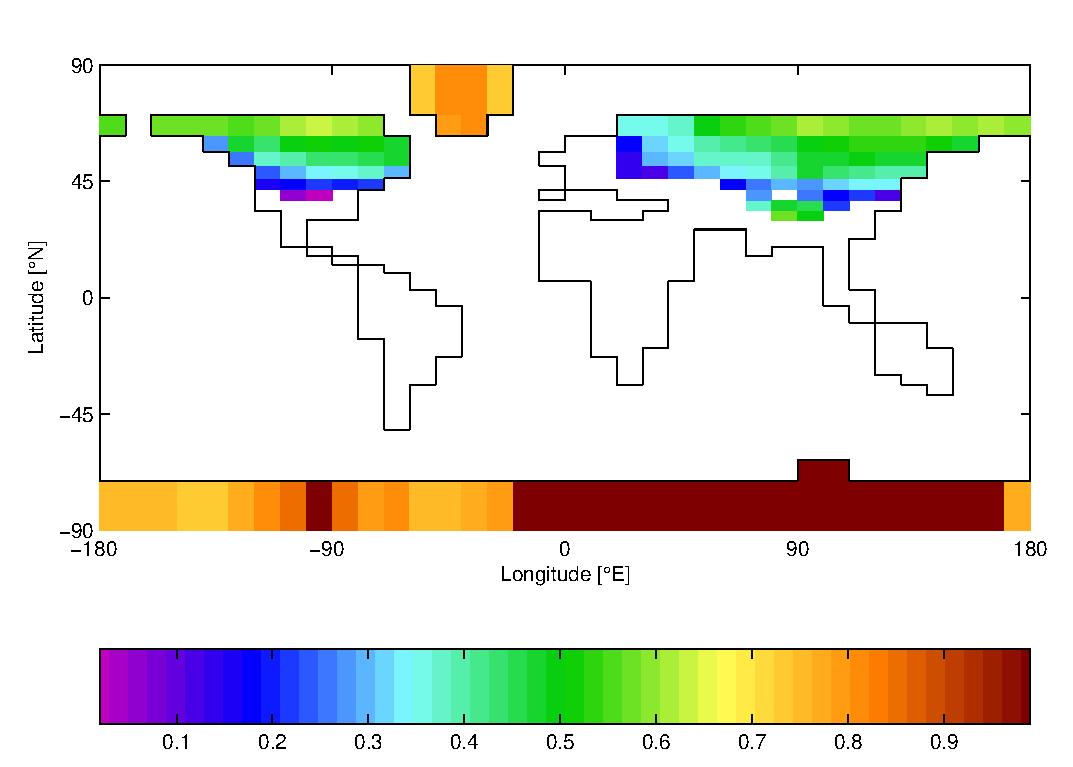
\includegraphics{snow.eps}}}
\caption{Annual average fractional snow cover}\label{snow}
\end{figure}

\section{Precipitation}

In {\em goin\_ents} there is an option to turn on or off an
alterative precipitation parameterizations than that used by
C-GOLDSTEIN. In C-GOLDSTEIN precipitation falls in a grid box if the
relative humidity of the air exceeds {\tt rmax}, a value you may
specify in {\em goin\_ents}. This is usually set to $0.85$ (a
relative humidity of $85$\%). The amount of precipitation falling is
the amount of moisture needed to be removed from the air to make the
relative humidity {\tt rmax} again. In ENTS, our alternative
function is based on the same principle but instead of instantaneous
precipitation, we relax the value of the relative humidity towards
{\tt rmax} with a timescale {\tt timepptn} (specified again in {\em
goin\_ents}), usually 5 days. The modified equation for
precipitation is given in equation (\ref{pptneqn}).
\begin{equation}\label{pptneqn}
P=\frac{1}{T}\frac{\rho_{a} h_a}{\rho_{o} \delta
t}(q_{a}-r_{max}q_{s}(T_{a}))
\end{equation}
Where $h_a$ is the height of the atmospheric boundary layer for
moisture, $T$ is {\tt timepptn} and $\delta t$ is the length of
the time step. This allows moisture to reach further into drier
areas of the globe. Figure \ref{pptn} shows the annual average
precipitation with this scheme.

\begin{figure}
\centerline{\scalebox{0.6}{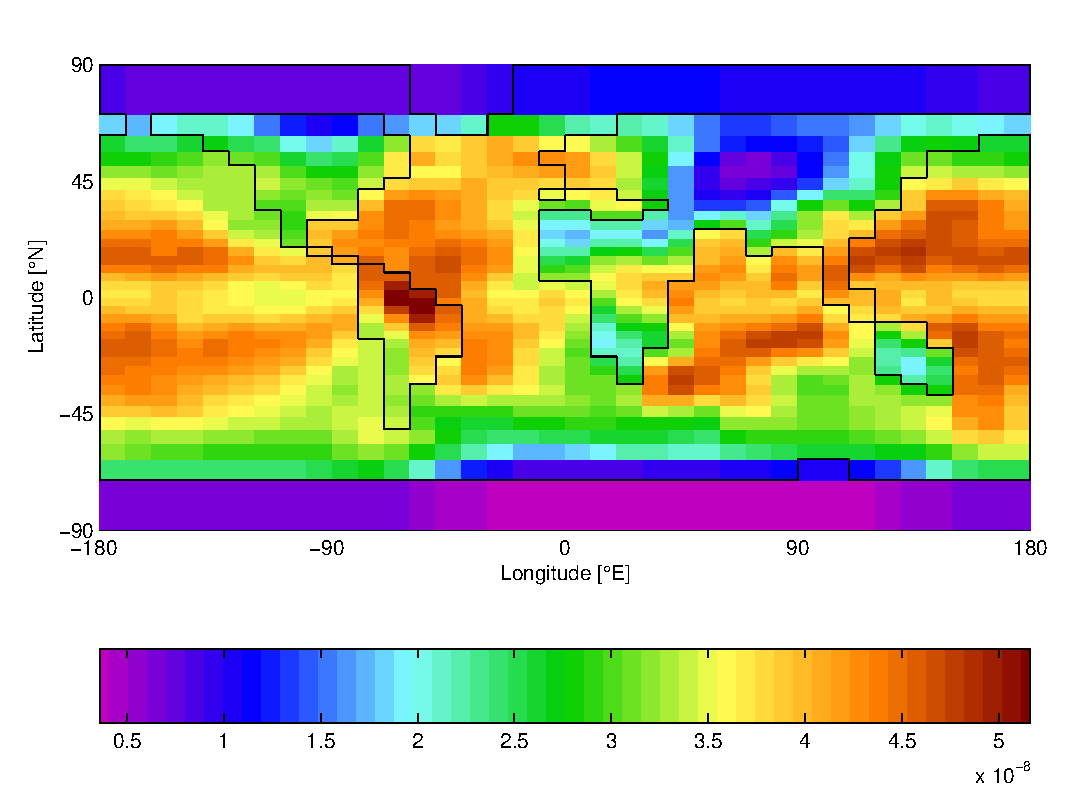
\includegraphics{pptn.eps}}}
\caption{Annual average precipitation in m/s}\label{pptn}
\end{figure}


\section{Seasonal winds}

Also included in the ENTS model are seasonal prescribed wind vector
fields for advecting moisture and temperature in the atmosphere and
seasonal prescribed surface wind speeds for calculating sensible
heat fluxes and evaporation. Seasonal winds change moisture movement
at different times of the year allowing the model to simulate
monsoons etc. more effectively. The prescribed fields come from NCEP
long term monthly mean data integrated vertically and weighted by
the amount of moisture at that level after \cite{Uvic}. These fields
are interpolated for each ocean timestep at the beginning of the run
using the interpolation scheme of Killworth (1996) \cite{Killworth}.
They can be switched off in favour of annual average fields by
changing {\tt seasonswitch} to 0 in {\em ents\_config.par}.

\section{Emissions}

ENTS also includes an option for forcing the model with carbon
emissions from a time series file located at {\em
genie-simpleland/data/emissions\_timeseries.dat}. When the emissions
forcing option is changed to `y' in {\em ents\_config.par} the model
adds carbon to the atmosphere. The first column in the {\em
emissions\_timeseries.dat} is the time in years from the beginning
of the run. The second column is carbon emissions in GtC/yr
(giga-tonnes of carbon per year). The model linearly interpolates
between the values in the timeseries file. This option maybe useful
to select if you wish to do global warming experiments once you have
spun the model up into a steady state.

\section{Sea-level change}

A simple calculation is performed by ENTS to get the change in
sea-level height from a reference number due to thermal expansion.
The reference number used in the calculation is that of global
average sea-water density that can be specified in {\em
sealevel\_config.par}. The variable name is {\tt rhoref}. The model
then calculates what the change in sea-level height is according to
the present global average sea-water density. The calculation
assumes that the ocean basins have vertical sides so any expansion
by the water is upwards and cannot spread onto or away from the
continents. To use this option effectively, run the model to a
steady state, use the final value of the global average ocean
density printed to a timeseries file in the model's output directory
(filename{\tt.sealevel}) and run the model through an emissions
scenario.

\section{Off-line testing}

ENTS may also be run `off-line'. When this option is selected in
{\em ents\_config.par} ENTS no longer sees the coupled model's
variables, it sees monthly data sets taken from NCEP i.e. the model
is forced with observed data. The observed fields it is forced with
are precipitation, relative humidity and air temperature. The
shortwave radiation flux entering the land still comes from the
coupled model however. This is a useful tuning and diagnostic tool
but while running the model in offline mode water is not conserved
globally. The ocean and atmosphere model still see precipitation as
calculated by the EMBM but evaporation and runoff for the land are
calculated from the NCEP data. This means water is not conserved
globally and generally the ocean gets progressively fresher. This
means ocean and atmosphere states when putting ENTS in offline mode
should not be used. However the ENTS restart file is useful for
getting realistic vegetation in continuing runs.

Figures of the vegetation and soil carbon in off-line mode are
shown in figure \ref{vegcarbontun} and figure \ref{soilcarbontun}
respectively. Observations of these two quantities are shown in
figures \ref{vegobs} and \ref{soilobs}

\begin{figure}
\centerline{\scalebox{0.6}{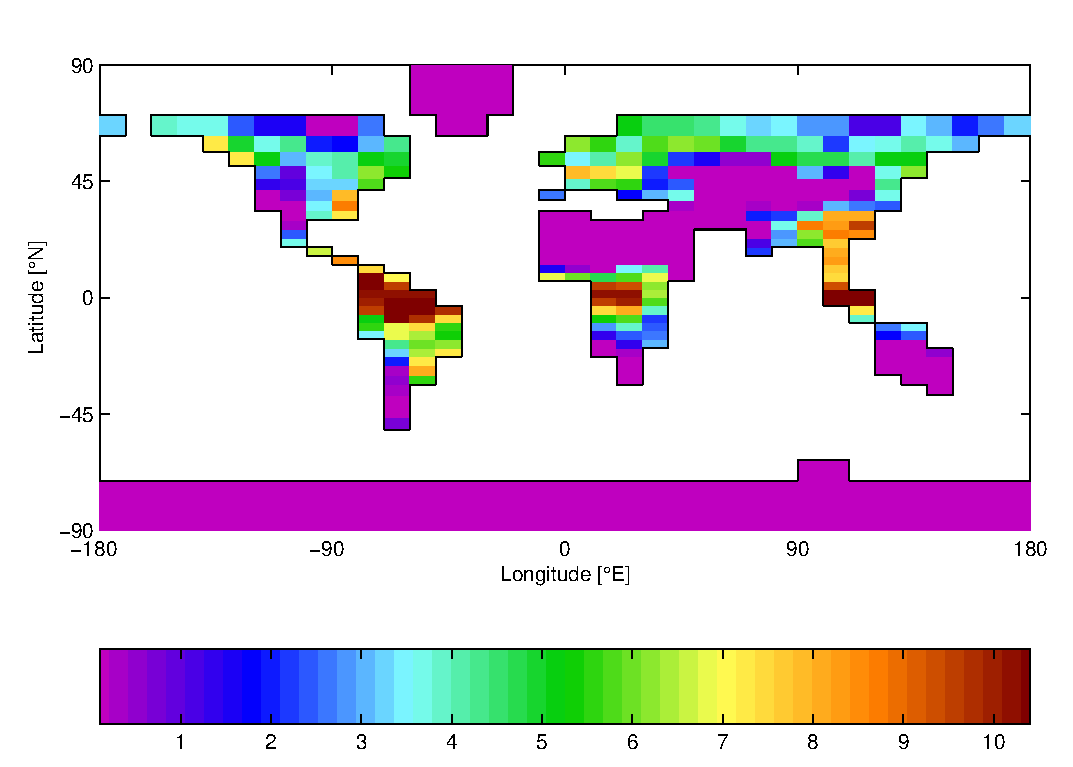
\includegraphics{vegcarbon_tun.eps}}}
\caption{Annual average vegetation carbon in off-line mode (kg
C/m$^{2}$)}\label{vegcarbontun}
\end{figure}

\begin{figure}
\centerline{\scalebox{0.6}{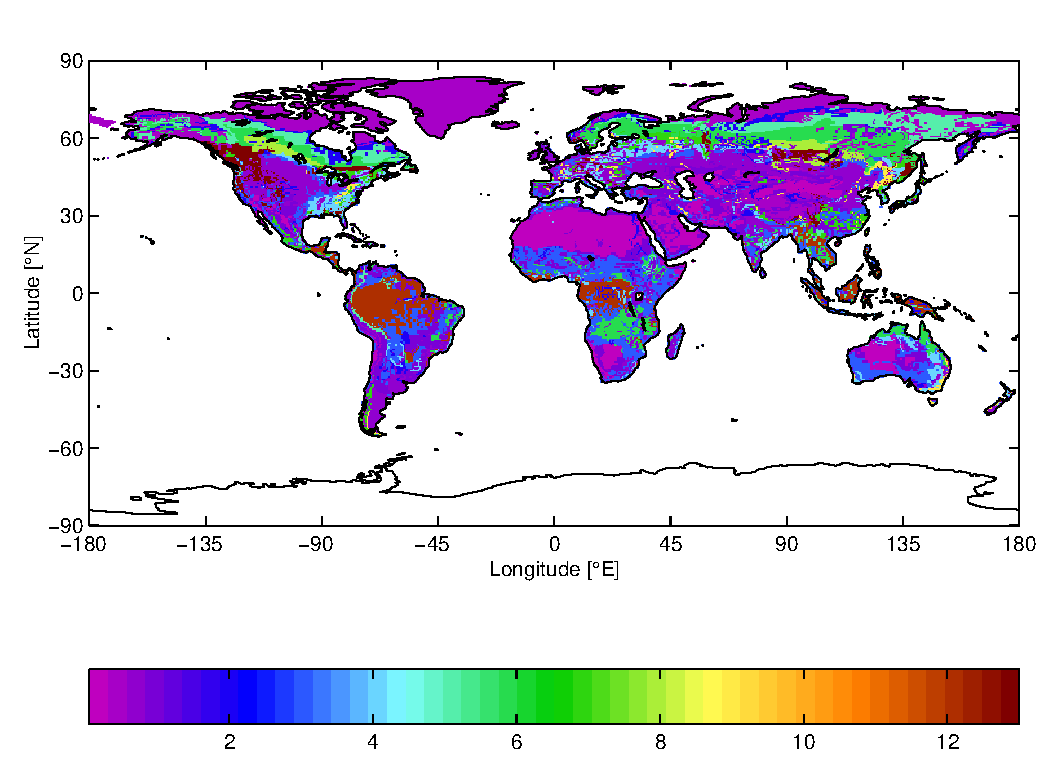
\includegraphics{vegcarbon_obs.eps}}}
\caption{Annual average vegetation carbon from observations (kg
C/m$^{2}$)}\label{vegobs}
\end{figure}

\begin{figure}
\centerline{\scalebox{0.6}{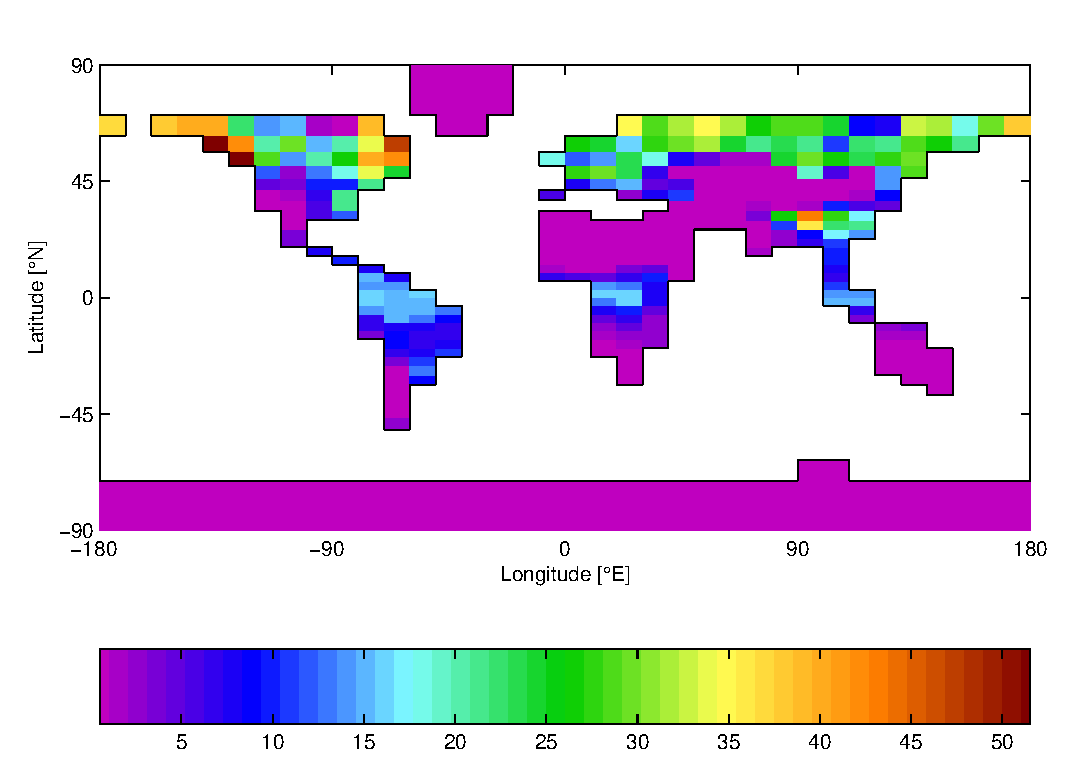
\includegraphics{soilcarbon_tun.eps}}}
\caption{Annual average soil carbon in off-line mode (kg
C/m$^{2}$)}\label{soilcarbontun}
\end{figure}

\begin{figure}
\centerline{\scalebox{0.6}{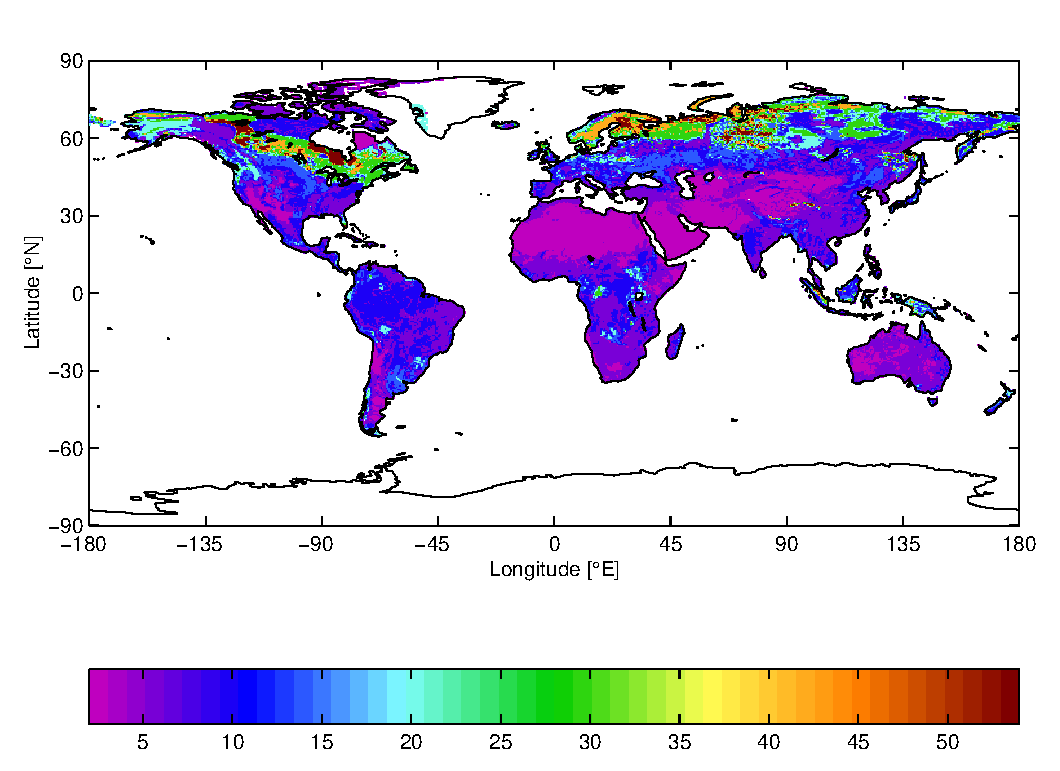
\includegraphics{soilcarbon_obs.eps}}}
\caption{Annual average soil carbon from observations (kg
C/m$^{2}$)}\label{soilobs}
\end{figure}

\section{Running the model with fixed vegetation}
There is a compile time option {\tt -Dfixedveg}. When this is
specified ENTS does not have a changing carbon scheme. The
vegetation carbon, soil carbon and vegetation fraction (determining
the land evaporation and land radiation fluxes) are fixed with an
annual average dataset for the duration of the run. You can set this
compiler option in {\em Makefile}.

\chapter{Compiling and running the model}

This section describes how to compile a version of the model that
includes C-GOLDSTEIN (ocean and EMBM atmosphere), BioGeM (ocean
biogeochemistry), AtChem (well mixed box atmospheric chemistry) and
ENTS to create a closed carbon cycle model, the executable
CBM-GOLDSTEIN.

\section{Compiling}

To compile the model, go to the directory {\em genie-cgoldstein}
and type the command

{\em make cbm\_goldstein}

This will compile all the subroutines that make up the complete
model. You may have some problems with compiler flags depending on
your machine's architecture and installed compilers. The flags for
the various machines are contained in the file {\em Makefile} in the
same directory. If you have problems compiling then comment out the
present `FLAGS = -r8 -o' with a `\#' and try another below it.
`FLAGS = -r8 -o' works with SGI machines and `FLAGS =
-xtypemap=real:64 -o' works with Sun workstations. After successful
compilation you should have an executable called {\em
cbm\_goldstein} sitting in the same directory.

\section{The goin and config files}

There is a goin file for C-GOLDSTEIN with BioGeM called {\em
goin\_bioents} which lives in the directory {\em genie-cgoldstein}
and a separate configuration file for ENTS in the directory {\em
genie-simpleland}. {\em goin\_bioents} sets the length of the run,
how often to write data, and the values of C-GOLDSTEIN's ocean and
atmosphere parameters. You can also alter the parameters that
control the precipitation, land roughness length and atmospheric
albedo.

The key parameters you may want to alter are the length of the run,
{\tt nsteps}, in ocean time steps (the number of ocean time steps
per year is given by the number the second row down, usually 100).
{\tt npstp} controls how often the model writes information to a
goout file (in ocean time steps). {\tt iwstp} tells the model how
often to write out a full dump, i.e. the current state of the model
that can be used for a restart from the same point. {\tt itstp}
tells the model how often to write to the time series files and {\tt
ianav} tells the model how often to calculate the model's annual
average state.

In the second row you can chose whether to start from a restart
file (put option `c') or to start the model from a homogenous
state and `spinup' the model (put option `n'). If you chose option
`c' then you must type the name of the restart file in the {\tt
input filename} row. The {\tt output filename} row specifies where
you want the model output to be written to.

For a proper explanation of this file please see the BioGeM and/or
C-GOLDSTEIN documentation.

The configuration file, {\em ents\_config.par} is hardwired into the
ENTS code so you must not change its name. In this file you can
specify how often ENTS is called in ocean timesteps, {\tt
msimpleland} (usually 5), the initial sizes of the global carbon
reservoirs in GtC (giga-tonnes of carbon) for vegetation ({\tt
Cveg\_ini}) and soil ({\tt Csoil\_ini}).

Next in the file follow a set of boolean logic switches. {\tt
orogswitch} turns the altitude effects on/off. {\tt snowswitch}
turns the snow albedo effect on/off. If {\tt offlineswitch} is set
to $1$ then the model reads in and is forced with NCEP data (to be
used for diagnostic and tuning purposes only). {\tt seasonswitch}
controls the form of the prescribed forcing fields. If set to $0$
then annual average fields are used. If set to $1$ the fields are
monthly means interpolated for each timestep.

The next line is whether or not to force the model with carbon
emissions from the time series file {\em emissions\_timeseries.dat}.
Select `y' or `n'. The last two rows control whether you want to
start the model from a DIFFERENT previous model dump and if yes, the
file's name and location.

In {\em goin\_bioents}, {\tt rmax} and {\tt timepptn} control the
precipitation scheme. {\tt rmax} is the relative humidity
(fractional) and {\tt timepptn} is the time scale in days. In {\em
sealevel\_config.par} {\tt rhoref} is the reference global ocean
density which is used to calculate change in sea-level height.

\section{To run the model}

Make sure you're in the directory {\em genie-cgoldstein} and have
produced the executable {\em cbm\_goldstein}. You also need to
create a directory {\em results} on the same level as the directory
{\em genie-cgoldstein}. After setting the desired parameters in {\em
goin\_bioents} and {\em ents\_config.par} you are ready to run the
model. To run the model type

{\em cbm\_goldstein $<$ goin\_bioents}

This should set the model running and printing information to the
screen. To print this information to a file instead of the screen
type

{\em cbm\_goldstein $<$ goin\_bioents $>$} filename


\section{Spinning the model up}

Producing a model state that looks like the pre-industrial world is
the usual starting point for transient experiments such as global
warming. Start the model from a homogenous state (the `n' option),
select the radiative CO$_{2}$ feedback to be turned on and run for
$5000$ years to obtain a steady state. Make sure you're restoring
the atmospheric CO$_{2}$ concentration to $278$ ppm to get the ocean
and atmospheric carbon inventories roughly correct. This is one of
biogem's options and can be set in {\em gem\_config\_atm.par}. Once
the model has reached a steady state you may like to check
everything is in equilibrium by turning the carbon restoring off in
biogem and running for a further period of time. This should produce
the pre-industrial steady state as a starter for transient runs. The
resulting vegetation state is shown in figure \ref{vegcarbon}.

Some figures of this final model state are shown. Figure
\ref{airtemp} shows the annual average air temperature. Figure
\ref{landtemp} shows the annual average land temperature.

\begin{figure}
\centerline{\scalebox{0.6}{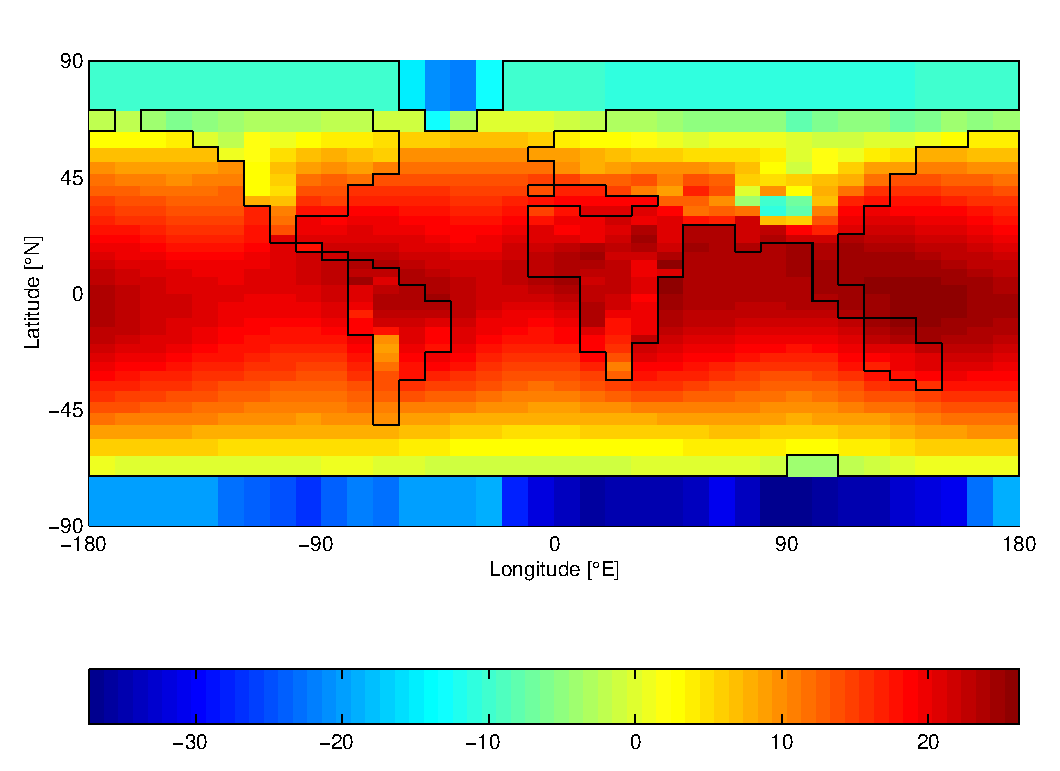
\includegraphics{airtemp.eps}}}
\caption{Annual average air temperature ($^{o}$C)}\label{airtemp}
\end{figure}

\begin{figure}
\centerline{\scalebox{0.6}{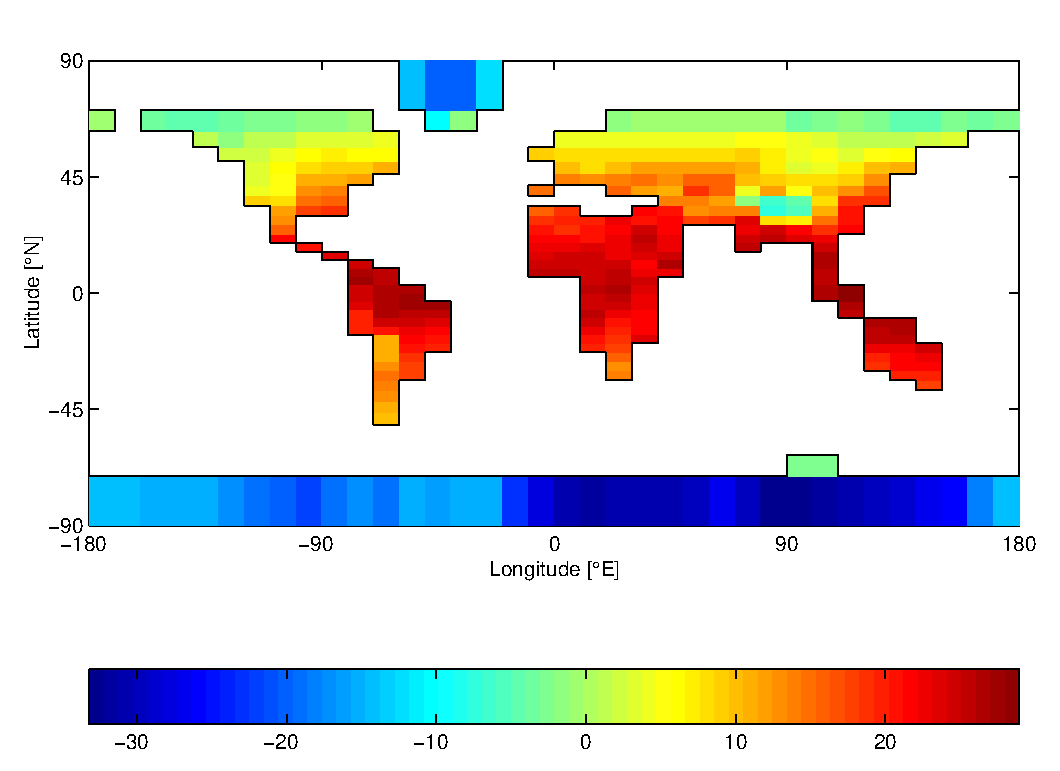
\includegraphics{landtemp.eps}}}
\caption{Annual average land temperature
($^{o}$C)}\label{landtemp}
\end{figure}

\begin{figure}
\centerline{\scalebox{0.6}{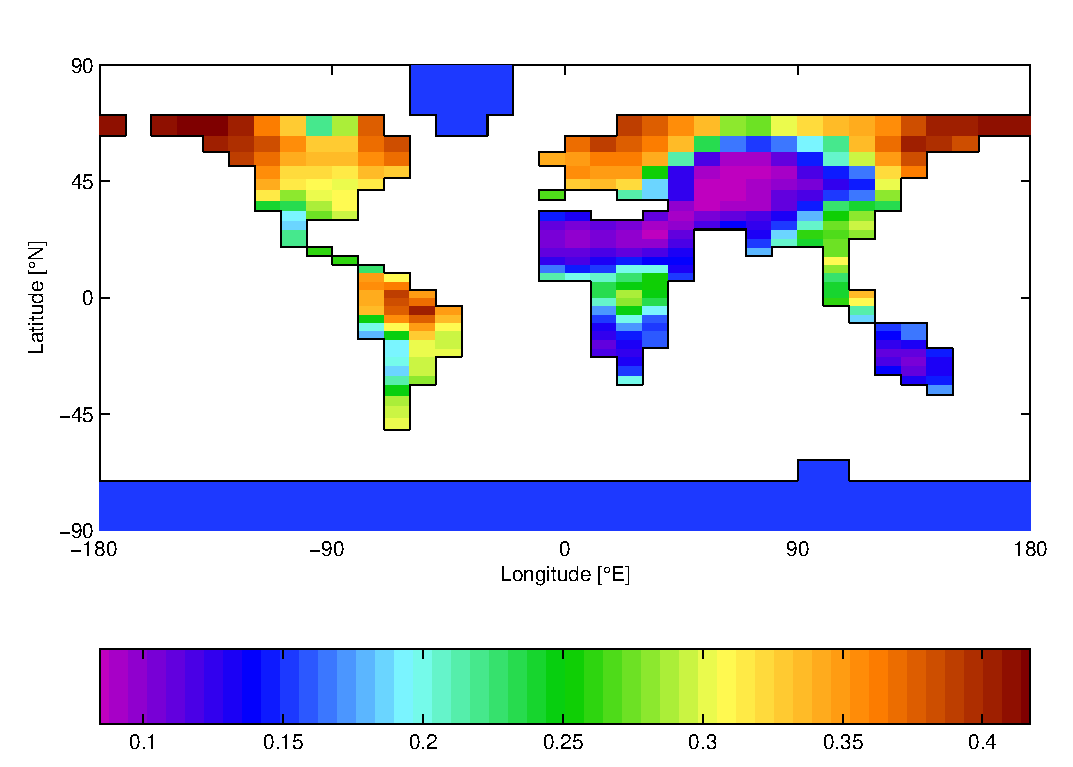
\includegraphics{water.eps}}}
\caption{Annual average water bucket height (m)}\label{water}
\end{figure}

\begin{figure}
\centerline{\scalebox{0.6}{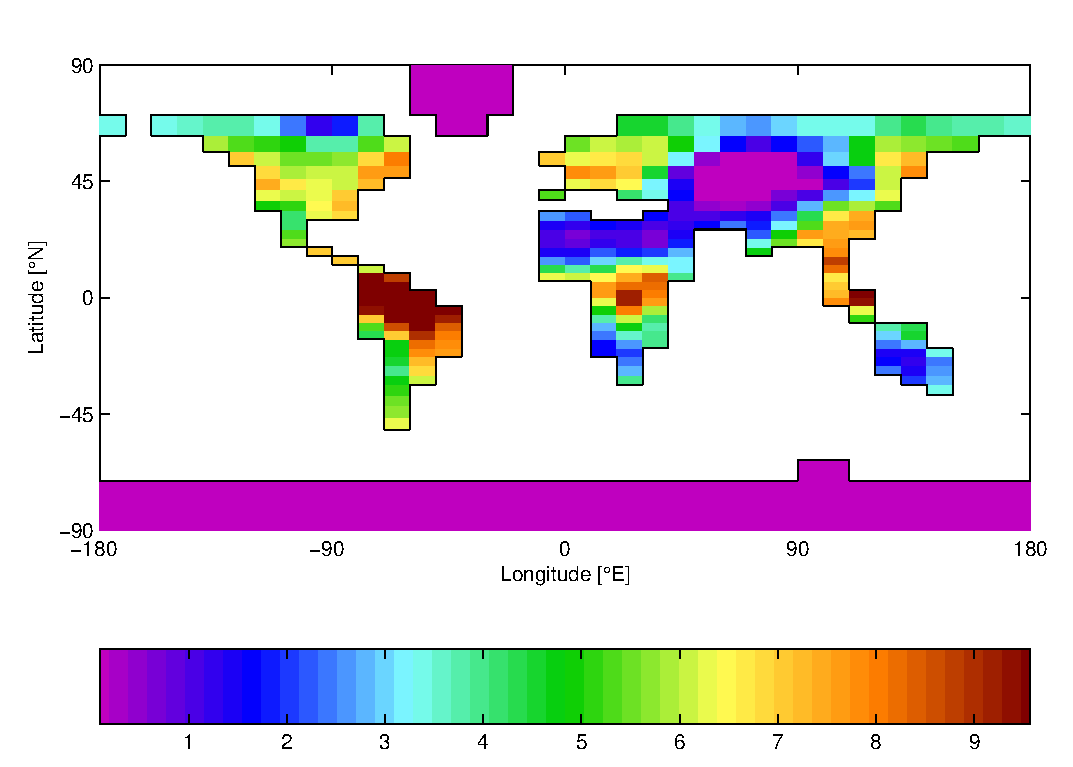
\includegraphics{vegcarbon.eps}}}
\caption{Annual average vegetation carbon (kg C/m$^{2}$) in the
coupled model. Orography effects have been turned
off.}\label{vegcarbon}
\end{figure}


\begin{figure}
\centerline{\scalebox{0.6}{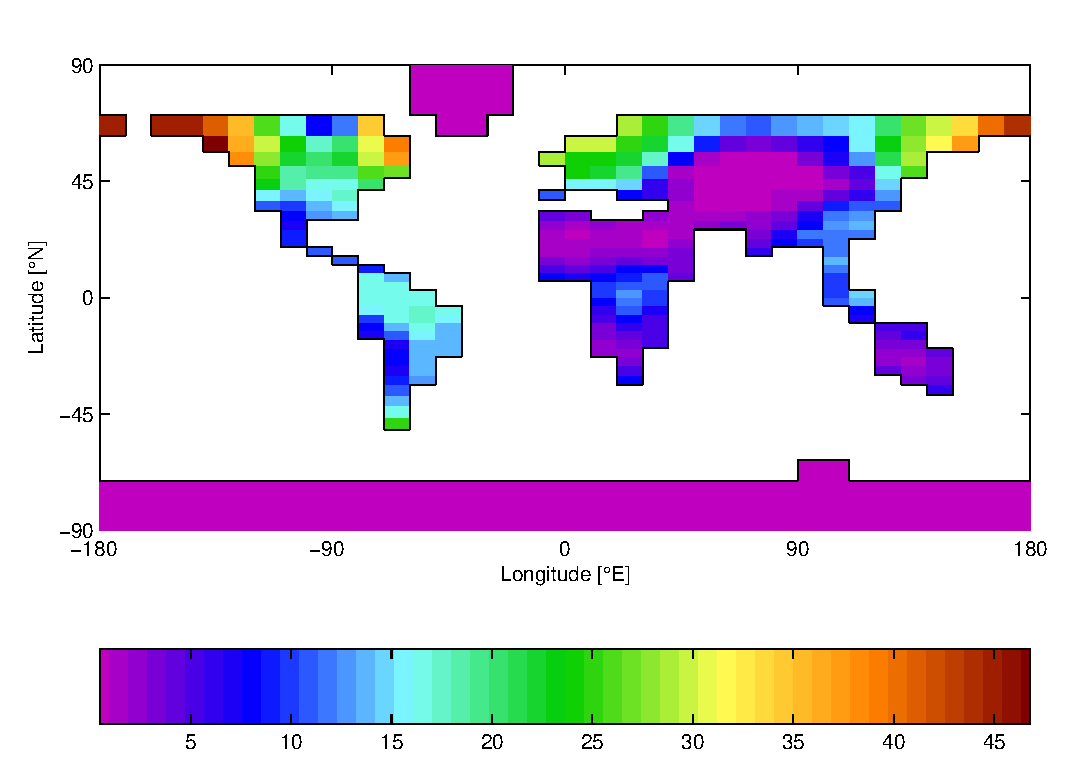
\includegraphics{soilcarbon.eps}}}
\caption{Annual average soil carbon (kg C/m$^{2}$) in the coupled
model. Orography effects have been turned off.}\label{soilcarbon}
\end{figure}

\section{Continuing a run from a model dump}

After you've finished spinning the model up and you're happy that
it's in a steady state you can use the model's output files as a
starting point for transient experiments. If you specified the model
output to have the name {\tt ini}, then the model dump files are:

{\tt ini.1} - C-GOLDSTEIN file

{\tt ini.1.biogem} - BioGeM file

{\tt ini.1.atchem} - AtChem file

{\tt ini.1.sland} - ENTS file

All these files need to be in a directory named {\em results} which
is the same directory that the model will send it's output to. It's
important to note that when specifying input and output names in
{\em goin\_bioents} that they are no more or no less than $7$
characters long for output file names and exactly $9$ characters
long for input file names. To continue a run using these files just
change the `n' to a `c' in the second row of {\em goin\_bioents} and
type a name to call the output files. All that remains is to set how
long you wish to run the model for and the various other parameters
in the goin file.

\chapter{Model outputs}

The model produces a number of output files in the directory {\em
results}. In this section the names of the files and the format in
which they produce the data will be given for the ENTS component
only. For C-GOLDSTEIN and BioGeM outputs please see those respective
user manuals.

\section{File names and data format}

\subsection{Two dimensional arrays}

The ENTS model produces a number of files that are output as one
long column of numbers of length $36 \times 36$. These files are of
one variable and have one value for each point of the C-GOLDSTEIN
grid (i.e. the grid is $36 \times 36$). Listed below are these files
with their units:

filename{\tt.lqavg} - The annual average amount of water in each
grid box (units meters).

filename{\tt.ltavg} - The annual average temperature of the land in
each grid box (units $^{o}$C).

filename{\tt.palbavg} - The annual average effective planetary
albedo for each grid box.

filename{\tt.snowavg} - The annual average fractional snow cover for
each grid box.

filename{\tt.albsavg} - The annual average surface albedo for each
grid box.

filename{\tt.runavg} - The annual average runoff for each grid box
(units m/s).

filename{\tt.pptnavg} - The annual average precipitation for each
grid box (units m/s).

filename{\tt.relhavg} - The annual average relative humidity for
each grid box.

filename{\tt.z0avg} - The annual average roughness length for each
grid box (units m).

filename{\tt.evaplavg} - The annual average evaporation for each
grid box (units m/s).


\subsection{Land dumps}

These are files that are produced to allow a perfect restart of the
model. They contain all the information the model needs to know to
calculate any other variable it needs, in other words this file
contains all the information about the model's state. There are two
files produced, both in the same format. These are
filename.$n${\tt.sland}, where $n$ is an integer from $0$ to $9$ and
filename{\tt.sland.avg}. Only filename$n$.{\tt.sland} allows perfect
restarts as this is a `snapshot' of the model's state at a
particular time. filename{\tt.sland.avg} is the complete model's
state annually averaged.

The data is printed in the following order (all in one column):

photosynthesis: $1$ to size of grid (should be $36 \times 36 =
1296$) in units of kg C /m$^2$/yr.

vegetation respiration: $1$ to size of grid in units of kg C
/m$^2$/yr.

leaf litter: $1$ to size of grid in units of kg C /m$^2$/yr.

soil respiration: $1$ to size of grid in units of kg C /m$^2$/yr.

vegetation carbon: $1$ to size of grid in units of kg C /m$^2$/yr.

soil carbon: $1$ to size of grid in units of kg C /m$^2$/yr.

land temperature: $1$ to size of grid in units of $^{o}$C.

land water: $1$ to size of grid in units of meters.

snow fraction: $1$ to size of grid, no units.

\subsection{Time series files}

ENTS produces a timeseries file of globally averaged quantities to
do with the carbon cycle. This file is written to every {\tt itstp}
ocean timesteps and is called filename{\tt.slandt}. The data is
formatted as follows:

column 1: time (in years from the start of the run)

column 2: vegetation carbon (GtC)

column 3: soil carbon (GtC)

column 4: atmospheric carbon (GtC)

column 5: vegetation fraction

column 6: CO$_{2}$ concentration (ppm)

column 7: photosynthesis (GtC/yr)

column 8: vegetation respiration (GtC/yr)

column 9: leaf litter (GtC/yr)

column 10: soil respiration (GtC/yr)

Another timeseries file of physical globally averaged quantities
\emph{over land} is produced. This file is written to every {\tt
itstp} ocean timesteps and is called filename{\tt.pslandt}. The data
is formatted as follows:

column 1: time (in years from the start of the run)

column 2: land temperature ($^o$C)

column 3: land water (m)

column 4: radiation flux to the atmosphere over land (W/m$^2$)

column 5: radiation flux to the land (W/m$^2$)

column 6: sensible heat flux to the atmosphere over land (W/m$^2$)

column 7: Net long wave heat flux to the atmosphere over land
(W/m$^2$)

column 8: Total evaporation (m/s)

column 9: Precipitation over land (m/s)

column 10: Relative humidity (fractional)

column 11: Soil field capacity (m)

column 12: Land surface albedo

column 13: Fractional snow cover

column 14: Roughness length (m)

ENTS also produces a timeseries file of average global ocean density
and sea-level height relative to the reference density {\tt rhoref}.
It is written to every {\tt itstp} ocean timesteps and is called
filename{\tt.sealevel}. The data is formatted as follows:

column 1: time (in years from the start of the run).

column 2: change in sea-level height relative to {\tt rhoref} (m).

column 3: global average ocean density (kg/m$^3$).

\subsection{Global mean air temperature}

This is actually calculated in c-goldstein but is added as one of
ENTS's outputs for convenience. The file is filename{\tt.gmairt}.
The file is a timeseries but is written to every {\tt ianav} ocean
timesteps rather than the usual {\tt itstp}. It has the following
format:

column 1: time (in years from the start of the present run)

column 2: global average air temperature ($^{o}$C).

\subsection{Annual average carbon reservoirs and fluxes}

This is a timeseries file that calculates the annual global average
carbon reservoir sizes and fluxes. This is written to every {\tt
ianav} ocean timesteps. The file has the extention {\tt .slavgt}.
This file is also very useful for tuning and finding out what's
going on in the global carbon cycle. It has the following format:

column 1: year from the beginning of the run

column 2: global annual average net photosynthesis (GtC/yr)

column 3: global annual average vegetation respiration (GtC/yr)

column 4: global annual average leaf litter (GtC/yr)

column 5: global annual average soil respiration (GtC/yr)

column 6: global annual average vegetation carbon (GtC)

column 7: global annual average soil carbon (GtC)

column 8: global annual average vegetation fractional cover

column 9: global annual average self shading fraction

column 10: global annual average atmospheric carbon (GtC)

column 11: global annual average ocean carbon (GtC) (only for
cbm\_goldstein)

The annual global average physical quantities for the land are
written in {\tt .pslavgt}. The file has the following format:

column 1: time (in years from the start of the run)

column 2: global annual average land temperature ($^o$C)

column 3: global annual average land water (m)

column 4: global annual average radiation flux to the atmosphere
over land (W/m$^2$)

column 5: global annual average radiation flux to the land (W/m$^2$)

column 6: global annual average sensible heat flux to the atmosphere
over land (W/m$^2$)

column 7: global annual average net long wave heat flux to the
atmosphere over land (W/m$^2$)

column 8: global annual average evaporation (m/s)

column 9: global annual average precipitation over land (m/s)

column 10: global annual average relative humidity (fractional)

column 11: global annual average soil field capacity (m)

column 12: global annual average land surface albedo

column 13: global annual average fractional snow cover

column 14: global annual average roughness length

\section{Plotting model output}

In the directory {\em genie-simpleland/plot} you will find some
matlab scripts that can be used to plot ENTS output. {\em
ents\_constants.m} and {\em ents\_mask.mat} are not plotting scripts
but are called by the other scripts as they contain the common
variables. {\em ents\_twoDarray.m} will plot the two dimensional
arrays. By typing {\tt ents\_twoDarray} in matlab you will be asked
to enter the run id and then be presented with the option of
plotting either water bucket fullness, land temperature, run off,
fractional snow cover or planetary albedo. {\em ents\_carbon.m} lets
you plot carbon flux fields i.e. photosynthesis, soil respiration or
carbon reservoirs and vegetated fraction. {\em ents\_timeseries.m}
produces an array of plots from {\tt .slandt}. {\em ents\_avgt.m}
will let you plot numbers and derived quantities from {\tt .slavgt}
including global annual average land carbon fluxes, carbon
inventories, net ecosystem productivity (NEP) and net primary
production (NPP). {\em ents\_pavgt.m} will let you plot global
annual average physical quantities from {\tt .pslavgt}. There is
also another script, {\em ents\_evap.m} that allows you to plot
evaporation, transpiration and evapotranspiration fields from the
file {\tt .evaplavg}. To plot sealevel change use {\em
ents\_sealevel.m}.

You need to specify the location of your model output in {\em
ents\_constants.m}. Where `path' is specified in this script put you
own file location.

\chapter{Tuning the model}

In this chapter we'll only discuss tuning the ENTS model and not the
other components of cbm\_goldstein. ENTS as it comes should produce
pre-industrial land carbon fluxes and land carbon inventories when
in offline mode. These numbers obtained from the 1995 IPCC report
are 550 GtC in vegetation carbon, 1500 GtC in soil carbon, 100
GtC/yr in net photosynthesis and 50 GtC/yr for vegetation
respiration, leaf litter and soil respiration. Tuning in offline
mode is made very easy as many of the feedbacks between the carbon
model and the climate are fixed. This makes the effect of changing
the carbon constants stored in {\em k\_constants.dat} almost linear
in response. With just one run you can calculate the values of the
$k$ constants that give you your desired fluxes i.e. the terrestrial
carbon flux equations reduce to

\begin{displaymath}
P=k_{18}K_{env}^P f_{\upsilon}
\end{displaymath}

\begin{displaymath}
R_{\upsilon}=\frac{k_{24}}{k_{25}}K_{env}^{R_{\upsilon}}C_{\upsilon}
\end{displaymath}

\begin{displaymath}
L=k_{26}C_{\upsilon}+\varepsilon(P-R_\upsilon)
\end{displaymath}

\begin{equation}
R_s=\frac{k_{29}}{k_{30}}K_{env}^{R_s}C_s
\end{equation}

Where the fluxes are global annual averages (GtC/yr) and
$C_{\upsilon}$ and $C_s$ are the global annual average reservoir
sizes (GtC) read from the file {\tt .slavgt}. After one run and a
rearrangement of the above equations to determine the values of the
environmental constants (the $K_{env}$) you can tune to any fluxes
and any reservoir sizes.

\chapter{Model code structure}

ENTS is structured much like C-GOLDSTEIN. Before the main time loop
ENTS is initialized by {\em setup\_ents.F}. This subroutine reads
from {\em goin\_bioents} and {\em ents\_config.par} and sets up the
initial state of the model. If the run is a continuing run then {\em
setup\_ents.F} calls another subroutine {\em in\_ents.f} which reads
in the model dump file. During the initialization stage, three other
subroutines are called: {\em setup\_emissions.f} is called from {\em
mains.F} and creates an array of carbon fluxes to feed the
atmosphere with throughout the run from the emissions time series
{\em emissions\_timeseries.dat}. Another is {\em ocean\_alb.f} which
is called from {\em radfor.F} that calculates the ocean albedo at
each latitude and {\tt istep} before the main time loop and {\em
field\_interp.f} which interpolates the prescribed monthly mean data
for every ocean timestep within one year.

During the main time loop in {\em mains.F} there are calls to two
different subroutines. One is a call to {\em surflux.F}, actually
part of C-GOLDSTEIN, that calculates heat and moisture fluxes and
updates these values. This subroutine is called every ocean
timestep. The second call is to {\em carbon.F} which calculate
carbon fluxes and updates reservoirs. This subroutine is called
every {\tt msimpleland} ocean time steps. These two subroutines form
the heart of ENTS.

There are four diagnostic subroutines. {\em annav\_diags.F}
calculates annual average timeseries and fields.{\em carbt\_diags.f}
and {\em physt\_diags.f} which calculate the globally averaged
`snapshot' quantities. {\em screen\_diags.f} calculates quantities
that are printed to the screen every {\tt npstp} ocean timesteps.

The last subroutine {\em out\_ents.f} is called every {\tt iwstp}
and outputs the full model dumps filename$n${\tt.sland.}

The remaining files are data sets and are found in the directory
{\em data}. {\em k\_constants.dat} is a list of constants used in
the carbon model. {\em orography.dat} are the elevations above
sea-level. {\em monthly\_uwind.silo, monthly\_vwind.silo} and {\em
monthly\_windspd.silo} are the $u$ and $v$ components of the wind
for each month and the wind speed for each month respectively.
{\em cloud\_albedo\_monthly.dat} contains the mean monthly cloud
albedo fields and all files prefixed with `{\em NCEP}' are the
files used to force the model in off-line mode.

Lastly {\em var\_ents.cmn} contains all the common blocks of the
model.

\chapter{Acknowledgments}

Mark Williamson, Tim Lenton and John Shepherd were supported by
the Tyndall Centre for climate change research. Andrew Yool was
supported by the GENIE project and Bob Marsh and Ben Adams were
supported by NERC funding.

Of the other components that make up {\em cbm-goldstein}, Andy
Ridgwell (BioGeM) was supported by the Tyndall Centre and Neil
Edwards is supported by the National Centres for Competence in
Research (Climate), Switzerland.

\begin{thebibliography}{10}
\bibitem{Lenton} T. M. Lenton (2000). Land and ocean carbon cycle
feedback effects on global warming in a simple Earth system model.
{\em Tellus} {\bf 52B}, 1159-1188.
\bibitem{Adams} B. Adams (2003). Modelling the Earth System. PhD
thesis, Heriot-Watt University.
\bibitem{Marsh and Edwards} N. Edwards and R. Marsh.
Uncertainities due to transport-parameter sensitivity in an
efficient 3-D ocean-climate model. {\em Climate Dynamics},
submitted.
\bibitem{Sellers} K. E. Trenberth (1992).{\em Climate sytem
modelling.} Cambridge University Press, 788pp.
\bibitem{Uvic} A. J. Weaver {\it et al.} (2001). The UVic Earth
system climate model: Model description, climatology, and
applications to past, present and future climates. {\em
Atmosphere-Ocean} {\bf 39}(4), 361-428.
\bibitem{Leuning} Leuning, R. (1995). A critical appraisal of a
combined stomatal-photosynthesis model for C3 plants.{\em Plant,
Cell and Environment} {\bf 18}: 339-355.
\bibitem{Dewar} Dewar, R. C. (1995). Interpretation of an empirical
model for stomatal conductance in terms of guard cell function.
{\em  Plant, Cell and Environment} {\bf 18}: 365-372.
\bibitem{Williamson} M. Williamson (2004). Analytic
solutions for the land temperature in an Earth system model of
intermediate complexity. Southampton Oceanography Centre internal
report No. 95.
\bibitem{Liou} K. N. Liou (1992). {\em Radiation and Cloud
Processes in the Atmosphere: Theory, Observation and Modelling.}
Oxford University Press, 487pp.
\bibitem{Matthews}  E. Matthews (1983). Global vegetation and land use:  new
high-resolution data bases for climate studies, {\em J. Clim.
Appl. Meteor.}, {\bf 22}, 474-487.
\bibitem{Ramanathan} B. P. Briegleb, P. Minnis, V. Ramanathan and
E. Harrison (1986). Comparison of regional clear-sky albedos
inferred from satellite observations and model comparisons. {\em
J. Clim. and App. Met.}, {\bf 25}, 214-226.
\bibitem{P+O} J. P. Peixoto and A. H. Oort (1991). {\em Physics of
Climate} AIP Press, 520pp.
\bibitem{Killworth} P. D. Killworth (1996). Time interpolation of
forcing fields in ocean models. {\em Journal of Physical
Oceanography}, {\bf 26}, 136-143.
\bibitem{cox} P. M. Cox, C. Huntingford and R. J. Harding (1998).
A canopy conductance and photosynthesis model for use in a GCM
land surface scheme. {\em Journal of Hydrology}, {\bf 212-213},
79-94.
\end{thebibliography}

\end{document}
